\chapter{The Supplied Test Problems}
\label{Sec:The supplied problems}

To verify that Flash-X works as expected and to debug changes in the code, we
have created a suite of standard test problems. Many of these problems have
analytical solutions that can be used to test the accuracy of the code. Most
of the problems that do not have analytical solutions produce
well-defined flow features that have been verified by experiments and are
stringent tests of the code. For the remaining problems, converged solutions,
which can be used to test the accuracy of lower resolution simulations, are
easy to obtain.  The test suite configuration code is included
with the Flash-X source tree (in the \code{Simulation/} directory), so it is easy
to configure and run Flash-X with any of these problems `out of the box.'
Sample runtime parameter files are also included. All the test
problems reside in the \code{Simulations} unit. The unit provides some
general interfaces most of which do not have general
implementations. Each application provides its own implementation for
these interfaces, for example, \code{Simulation\_initBlock}. The
exception is \code{Simulation\_initSpecies}, which provides general
implementations for different classes of problems. 

\section{Hydrodynamics Test Problems}
These problems are primarily designed to test the functioning of the
hydrodynamics solvers within \flashx.

\subsection{Sod Shock-Tube}
\label{Sec:SimulationSod}

The Sod problem (Sod 1978) is a one-dimensional flow
discontinuity problem that provides a good test of a compressible code's
ability to capture shocks and contact discontinuities with a small number of
cells and to produce the correct profile in a rarefaction. It also
tests a code's ability to correctly satisfy the Rankine-Hugoniot shock
jump conditions. When implemented at an angle to a multidimensional grid,
it can be used to detect irregularities in planar discontinuities produced
by grid geometry or operator splitting effects.

We construct the initial conditions for the Sod problem by establishing a
planar interface at some angle to the $x$- and $y$-axes. The fluid is initially
at rest on either side of the interface, and the density and pressure jumps
are chosen so that all three types of nonlinear, hydrodynamic waves
(shock, contact, and rarefaction) develop.
To the ``left'' and ``right'' of the interface we have
\begin{equation}
\begin{array}{lclcclcl}
\rho_{\rm L} &=& 1.0 &   &   & \rho_{\rm R} &=& 0.125\\
p_{\rm L}    &=& 1.0 &   &   & p_{\rm R}    &=& 0.1
\end{array}
\end{equation}
The ratio of specific heats $\gamma$ is chosen to be 1.4 on both sides of
the interface.

In Flash-X, the Sod problem (\code{Sod}) uses the runtime parameters
listed in \tblref{Tab:Sod parameters} in addition to those supplied
by default with the code. For this problem we use the \code{Gamma} equation of
state \childunit and set \rpi{Eos/gamma} to 1.4. The default values listed
in \tblref{Tab:Sod parameters} are appropriate to a shock with
normal parallel to the $x$-axis that initially intersects that axis
at $x=0.5$ (halfway across a box with unit dimensions).
\begin{table}[!ht]

\caption{ Runtime parameters used with the
\code{Sod} test problem.}
\label{Tab:Sod parameters} 
\begin{center}
\begin{tabular}{lllp{3in}}
Variable    & Type      & Default   & Description\\
\hline
\code{sim\_rhoLeft}    & real      & 1     & Initial density to the
                          left of the interface
                          ($\rho_{\rm L}$)\\
\code{sim\_rhoRight}& real     & 0.125     & Initial density to the
                          right ($\rho_{\rm R}$)\\
\code{sim\_pLeft}  & real      & 1     & Initial pressure to the
                          left ($p_{\rm L}$)\\
\code{sim\_pRight} & real      & 0.1       & Initial pressure to the
                          right ($p_{\rm R}$)\\
\code{sim\_uLeft}  & real      & 0     & Initial velocity
                          (perpendicular to interface)
                          to the left ($u_{\rm L}$)\\
\code{sim\_uRight} & real      & 0     & Initial velocity
                          (perpendicular to interface)
                          to the right ($u_{\rm R}$)\\
\code{sim\_xangle}   & real      & 0     & Angle made by interface
                          normal with the $x$-axis
                          (degrees)\\
\code{sim\_yangle}   & real      & 90        & Angle made by interface
                          normal with the $y$-axis
                          (degrees)\\
\code{sim\_posn} & real      & 0.5       & Point of intersection between
                          the interface plane and the
                          $x$-axis\\
\hline
\end{tabular}
\end{center}

\end{table}

\begin{figure}
\begin{center}
{\leavevmode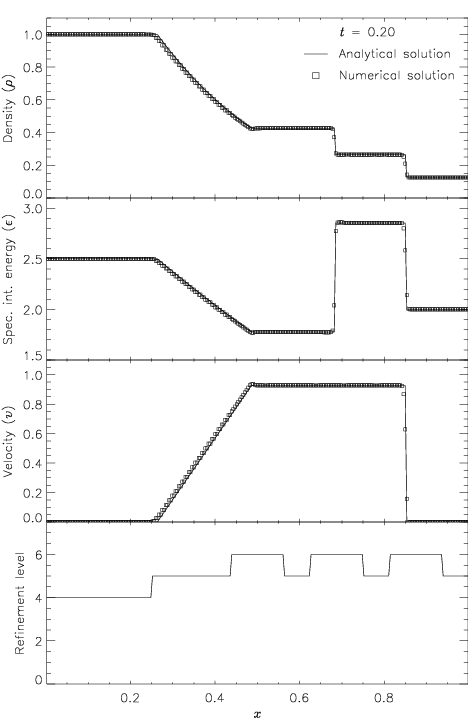
\includegraphics[width=5in]{Sod_single}}
\end{center}
\caption{\label{Fig:Sod single} Comparison of numerical and analytical
solutions to the Sod problem. A 2D grid with six levels of refinement
is used. The shock normal is parallel to the $x$-axis.
}
\end{figure}
\begin{figure}
\begin{center}
{\leavevmode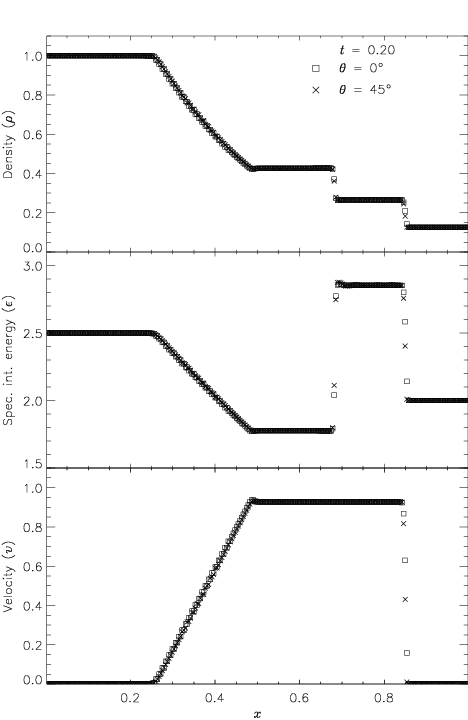
\includegraphics[width=5in]{Sod_compare}}
\end{center}
\caption{\label{Fig:Sod comparison} Comparison of numerical
solutions to the Sod problem for two different angles ($\theta$) of the
shock normal relative to the $x$-axis. A 2D grid with six levels of
refinement is used.
}
\end{figure}

\figref{Fig:Sod single} shows the result of running the Sod problem
with Flash-X on a two-dimensional grid with the analytical solution
shown for comparison. The hydrodynamical algorithm used here is the
directionally split piecewise-parabolic method (PPM) included with
Flash-X. In this run the shock normal is chosen to be parallel to the
$x$-axis. With six levels of refinement, the effective grid size at
the finest level is $256^2$, so the finest cells have width
0.00390625. At $t=0.2$, three different nonlinear waves are present:
a rarefaction between $x = 0.263$ and $x = 0.486$, a contact
discontinuity at $x = 0.685$, and a shock at $x = 0.850$. The two
discontinuities are resolved with approximately two to three cells
each at the highest level of refinement, demonstrating the ability
of PPM to handle sharp flow features well. Near the contact
discontinuity and in the rarefaction, we find small errors of about
$1-2\%$ in the density and specific internal energy, with similar
errors in the velocity inside the rarefaction. Elsewhere, the
numerical solution is close to exact; no oscillations are present.

\figref{Fig:Sod comparison} shows the result of running the Sod
problem on the same two-dimensional grid with different shock
normals: parallel to the $x$-axis ($\theta=0^\circ$) and along the
box diagonal ($\theta=45^\circ$). For the diagonal solution, we have
interpolated values of density, specific internal energy, and
velocity to a set of 256 points spaced exactly as in the $x$-axis
solution. This comparison shows the effects of the second-order
directional splitting used with Flash-X on the resolution of shocks.
At the right side of the rarefaction and at the contact
discontinuity, the diagonal solution undergoes slightly larger
oscillations (on the order of a few percent) than the $x$-axis
solution. Also, the value of each variable inside the discontinuity
regions differs between the two solutions by up to 10\%. However,
the location and thickness of the discontinuities is the same for
the two solutions. In general, shocks at an angle to the grid are
resolved with approximately the same number of cells as shocks
parallel to a coordinate axis.

\figref{Fig:Sod density} presents a colormap plot of the density at
$t=0.2$ in the diagonal solution together with the block structure
of the AMR grid. Note that regions surrounding the discontinuities
are maximally refined, while behind the shock and contact
discontinuity, the grid has de-refined, because the second
derivative of the density has decreased in magnitude. Because
zero-gradient outflow boundaries were used for this test, some
reflections are present at the upper left and lower right corners,
but at $t=0.2$ these have not yet propagated to the center of the
grid.

\begin{figure}[!ht]
\begin{center}
{\leavevmode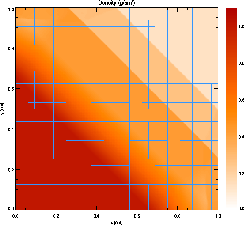
\includegraphics[width=3in]{Sod_2d_density}}
\end{center}
\caption{\label{Fig:Sod density} Density in the diagonal 2D Sod problem
with six levels of refinement at $t=0.2$. The outlines of AMR blocks are
shown (each block contains $8\times8$ cells).
}
\end{figure}


\subsection{Variants of the Sod Problem in Curvilinear Geometries}
\label{Sec:SimulationSodCurvi}
Variants of the \code{Sod} problems can be set up in in various 
geometries in order to test the handling of non-Cartesion geometries.

\begin{itemize}
\item
An axisymmetric variant of the Sod problem can be configured by
setting up the regular \code{Sod} simulation with 
\code{./setup Sod -auto -2d -geometry=cylindrical} and using runtime parameters
that include \code{geometry = "cylindrical"}. 
Use \code{sim_xangle = 0}
to configure an initial shock front that is shaped like a cylinder.
Results as in those discussed in Toro 1999 can be obtained.
\item
A spherically symmetric variant of the Sod problem can be configured by
setting up the regular \code{Sod} simulation with 
\code{./setup Sod -auto -1d -geometry=spherical} and using runtime parameters
that include \code{geometry = "spherical"}.
Again results as in those discussed in Toro 1999 can be obtained.
\item
To test the behavior of Flash-X solutions when the physical symmetry of the
problem does not match the geometry of the simulation,
a separate simulation is provided under the name \code{SodSpherical}.
To use this, configure with \code{./setup SodSpherical -auto -2d -geometry=spherical}
 and using runtime parameters
that include \code{geometry = "spherical"}.
As a 2D setup, \code{SodSpherical} represents physically axisymmetric
initial conditions in spherical coordinates. The physical problem
can be chosen to be the same as in the previous case with cylindrical \code{Sod}.
Again results as in those discussed in Toro 1999 can be obtained.
\item
The \code{SodSpherical} setup can also configured in 1D and will act
like the 1D \code{Sod} setup in that case.
\end{itemize}


\subsection{Sedov Explosion}
\label{Sec:SimulationSedov}

The Sedov explosion problem (Sedov 1959) is another purely hydrodynamical
test in which we check the code's ability to deal with strong shocks
and non-planar symmetry. The problem involves the self-similar evolution
of a cylindrical or
spherical blast wave from a delta-function initial pressure perturbation
in an otherwise homogeneous medium. 
We provide two different ways to generate the initial conditions:
\begin{enumerate}
\item
We deposit a quantity of energy $E=1$ into a
small region of radius $\delta r$ at the center of the grid.
The pressure inside this volume $p_0'$ is given by
\begin{equation}
p_0' = {3(\gamma-1)E\over(\nu+1)\pi\,\delta r^\nu}\ ,
\end{equation}
\noindent where $\nu=2$ for cylindrical geometry and $\nu=3$ for spherical
geometry. 
\item
We initialize from a precomputed pseudo-analytical solution by reading
in a 1D profile.
\end{enumerate}

We set the ratio of specific heats $\gamma=1.4$.
In running this problem we choose $\delta r$ to be 3.5
times as large as the finest adaptive mesh resolution in order to minimize
effects due to the Cartesian geometry of our grid.
The density
is set equal to $\rho_0=1$ everywhere, and the
pressure is set to a small value $p_0=10^{-5}$ everywhere but in the center
of the grid.
The fluid is initially at rest.
In the self-similar blast wave that develops for $t>0$, the
density, pressure, and radial velocity are all functions of
$\xi \equiv r/R(t)$, where
\begin{equation}
R(t) = C_\nu(\gamma) \left({Et^2\over \rho_0}\right)^{1/(\nu+2)}\ .
\end{equation}
\noindent Here $C_\nu$ is a
dimensionless constant depending only on $\nu$ and $\gamma$; for
$\gamma=1.4$, $C_2 \approx C_3 \approx 1$ to within a few percent.
Just behind the shock front at $\xi = 1$ the analytical solution is
\begin{eqnarray}
\nonumber
\rho = & \rho_1\,\, \equiv & {\gamma+1\over\gamma-1}\rho_0 \\
p    = & p_1\,\,    \equiv & {2\over\gamma+1}\rho_0 u^2 \\
\nonumber
v    = & v_1\,\,    \equiv & {2\over\gamma+1}u\ ,
\end{eqnarray}
\noindent where $u \equiv dR/dt$ is the speed of the shock wave. Near the
center of the grid,
\begin{eqnarray}
\nonumber
\rho(\xi)/\rho_1 & \propto & \xi^{\nu/(\gamma-1)} \\
p(\xi)/p_1       & =       & {\rm constant}\ \\
\nonumber
v(\xi)/v_1       & \propto & \xi \ .
\end{eqnarray}

\begin{figure}
\begin{center}
{\leavevmode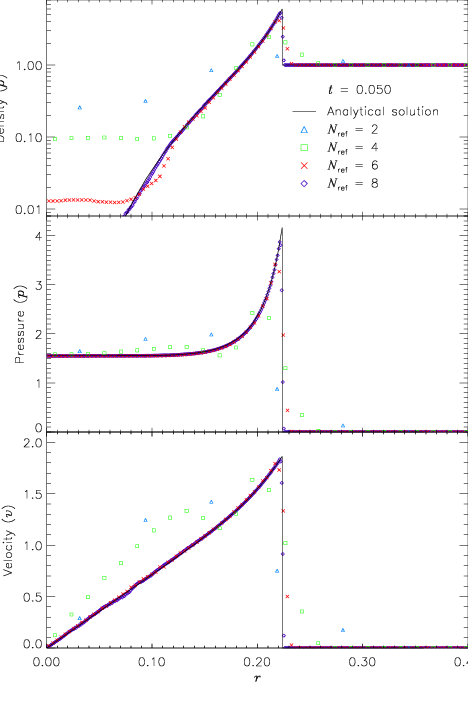
\includegraphics[width=5in]{Sedov_2d_compare}}
\end{center}
\caption{\label{Fig:Sedov compare} Comparison of numerical and analytical
solutions to the Sedov problem in two dimensions. Numerical solution values
are averages in radial bins at the finest AMR grid resolution $N_{\rm ref}$ in each run.
}
\end{figure}
\figref{Fig:Sedov compare} shows density, pressure, and velocity
profiles in the two-dimensional, cylindrical Sedov problem at
$t=0.05$. Solutions obtained with Flash-X on grids with 2, 4, 6, and 8
levels of refinement are shown in comparison with the analytical
solution. In this figure we have computed average radial profiles in
the following way. We interpolated solution values from the
adaptively gridded mesh used by Flash-X onto a uniform mesh having the
same resolution as the finest AMR blocks in each run. Then, using
radial bins with the same width as the cells in the uniform mesh, we
binned the interpolated solution values, computing the average value
in each bin. At low resolutions, errors show up as density and
velocity overestimates behind the shock, underestimates of each
variable within the shock, and a very broad shock structure.
However, the central pressure is accurately determined, even for two
levels of refinement. Because the density goes to a finite value
rather than to its correct limit of zero, this corresponds to a
finite truncation of the temperature (which should go to infinity as
$r\rightarrow 0$).  This error results from depositing the initial
energy into a finite-width region rather than starting from a delta
function. As the resolution improves and the value of $\delta r$
decreases, the artificial finite density limit also decreases; by
$N_{\rm ref}=6$ it is less than 0.2\% of the peak density. Except
for the $N_{\rm ref}=2$ case, which does not show a well-defined
peak in any variable, the shock itself is always captured with about
two cells. The region behind the shock containing 90\% of the
swept-up material is represented by four cells in the $N_{\rm
ref}=4$ case, 17 cells in the $N_{\rm ref}=6$ case, and 69 cells for
$N_{\rm ref}=8$. However, because the solution is self-similar, for
any given maximum refinement level, the structure will be four cells
wide at a sufficiently early time. The behavior when the shock is
under-resolved is to underestimate the peak value of each variable,
particularly the density and pressure.

\figref{Fig:Sedov refinement} shows the pressure field in the
8-level calculation at $t=0.05$ together with the block refinement
pattern. Note that a relatively small fraction of the grid is
maximally refined in this problem. Although the pressure gradient at
the center of the grid is small, this region is refined because of
the large temperature gradient there. This illustrates the ability
of \Paramesh to refine grids using several different variables at
once.
\begin{figure}[!ht]
\begin{center}
{\leavevmode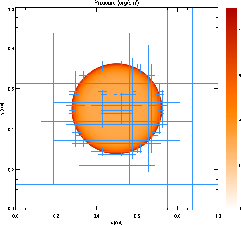
\includegraphics[width=3in]{Sedov_pressure}}
\end{center}
\caption{\label{Fig:Sedov refinement} Pressure field in the
2D Sedov explosion problem with 8 levels of refinement at $t=0.05$.
The outlines of the AMR blocks are overlaid on the pressure colormap.
}
\end{figure}


%In \figref{Fig:Sedov convergence}
%we plot the pressure error norm ([\eqref{Eqn:L1 error norm}]) for
%these results as a function of the effective number of cells.
%Note that here we are measuring the accuracy of the code, rather than
%the self-convergence rate, because we measure errors against the
%analytical solution. ...
%
%\begin{figure}
%\begin{center}
%%{\leavevmode\includegraphics[width=5in]{Sedov_2d_conv}}
%\end{center}
%\caption{\label{Fig:Sedov convergence} Convergence of the
%pressure in the two-dimensional \code{sedov} test problem.
%}
%\end{figure}

We have also run Flash-X on the spherically symmetric Sedov problem in
order to verify the code's performance in three dimensions. The
results at $t=0.05$ using five levels of grid refinement are shown
in \figref{Fig:Sedov 3D single}. In this figure we have plotted the
average values as well as the root-mean-square (RMS) deviations from
the averages. As in the two-dimensional runs, the shock is spread
over about two cells at the finest AMR resolution in this run. The
width of the pressure peak in the analytical solution is about 1~1/2
cells at this time, so the maximum pressure is not captured in the
numerical solution. Behind the shock the numerical solution average
tracks the analytical solution quite well, although the Cartesian
grid geometry produces RMS deviations of up to 40\% in the density
and velocity in the de-refined region well behind the shock. This
behavior is similar to that exhibited in the two-dimensional problem
at comparable resolution.
\begin{figure}
\begin{center}
{\leavevmode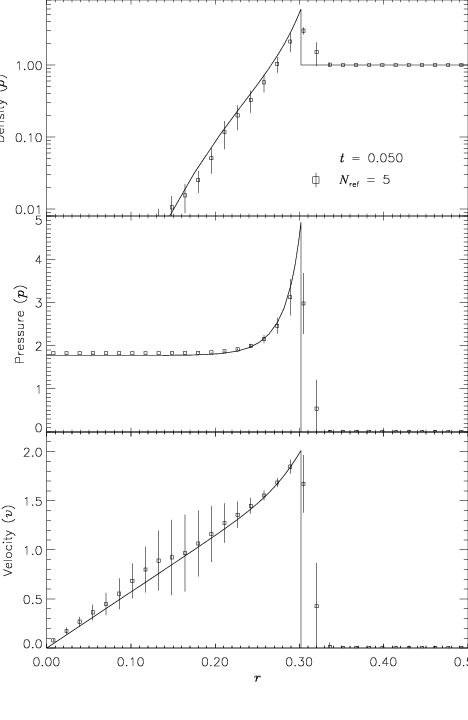
\includegraphics[width=5in]{Sedov_3d_single}}
\end{center}
\caption{\label{Fig:Sedov 3D single} Comparison of numerical and analytical
solutions versus radius $r$ to the spherically symmetric Sedov problem. A 3D grid with
five levels of refinement is used.
}
\end{figure}

The additional runtime parameters supplied with the \code{Sedov}
problem are listed in \tblref{Tab:Sedov parameters}. This problem is
configured to use the perfect-gas equation of state (\code{Gamma})
with \rpi{Eos/gamma} set to 1.4.  It is simulated in a unit-sized box.

\begin{table}

\caption{ Runtime parameters used with the
\code{Sedov} test problem.}
\label{Tab:Sedov parameters} 
\begin{center}
\begin{tabular}{lllp{3in}}
Variable    & Type      & Default   & Description\\
\hline
\code{sim\_pAmbient}& real     & $10^{-5}$ & Initial ambient pressure
                          ($p_0$)\\
\code{sim\_rhoAmbient}
        & real      & 1     & Initial ambient density
                          ($\rho_0$)\\
\code{sim\_expEnergy}
        & real      & 1     & Explosion energy ($E$)\\
\code{sim\_rInit}  & real      & 0.05      & Radius of initial pressure
                          perturbation ($\delta r$)\\
\code{sim\_xctr} & real      & 0.5       & $x$-coordinate of explosion
                          center\\
\code{sim\_yctr} & real      & 0.5       & $y$-coordinate of explosion
                          center\\
\code{sim\_zctr} & real      & 0.5       & $z$-coordinate of explosion
                          center\\
\code{sim\_nSubZones} & integer & 7 & Number of sub-cells in cells for applying the 1D profile \\
\hline
\end{tabular}
\end{center}

\end{table}
\subsection{Isentropic Vortex}
\label{Sec:SimulationIsentropicVortex}

The two-dimensional isentropic vortex problem is often used as a
benchmark for comparing numerical methods for fluid dynamics. The
flow-field is smooth (there are no shocks or contact discontinuities)
and contains no steep gradients, and the exact solution is known. It
was studied by Yee, Vinokur, and Djomehri (2000) and by Shu (1998). In
this subsection the problem is described, the Flash-X control parameters
are explained, and some results demonstrating how the problem can be
used are presented.

The simulation domain is a square, and the center of the vortex is
located at $(x_{ctr}, y_{ctr})$. The flow-field is defined in
coordinates centered on the vortex center $(x' = x - x_{ctr}, y' = y
- y_{ctr})$ with $r^2 = {x'}^2 + {y'}^2$. The domain is periodic, but
it is assumed that off-domain vortexes do not interact with the
primary; practically, this assumption can be
satisfied by ensuring that the simulation domain is large enough for a
particular vortex strength. We find that a domain size of $10 \times
10$ (specified through the \code{Grid} runtime parameters \rpi{Grid/xmin},
\rpi{Grid/xmax}, \rpi{Grid/ymin}, and \rpi{Grid/ymax}) is sufficiently large for a
vortex strength (defined below) of~5.0. In the initialization below,
$x'$ and $y'$ are the coordinates with respect to the nearest vortex
in the periodic sense.

The ambient conditions are given by $\rho_\infty$, $u_\infty$,
$v_\infty$, and $p_\infty$, and the non-dimensional ambient temperature
is $T^*_\infty = 1.0$. Using the equation of state, the (dimensional)
$T_\infty$ is computed from $p_\infty$ and
$\rho_\infty$. Perturbations are added to the velocity and
nondimensionalized temperature, $u = u_\infty + \delta u$, $v =
v_\infty + \delta v$, and $T^* = T^*_\infty + \delta T^*$ according to
\begin{eqnarray}
\label{Eqn:isentropic_three}
\delta u &=&
-y' {\frac {\beta} {2 \pi}} \exp \left( {\frac {1-r^2} {2}} \right) \\
\delta v &=&
 x' {\frac {\beta} {2 \pi}} \exp \left( {\frac {1-r^2} {2}} \right) \\
\delta T^* &=&
- { \frac {(\gamma - 1 ) \beta}  {8 \gamma \pi^2}} \exp \left( {1-r^2}
\right)~,
\end{eqnarray}
where $\gamma=1.4$ is the ratio of specific heats and $\beta=5.0$ is a
measure of the vortex strength. The temperature and density are then given by
\begin{eqnarray}
T &=& {\frac{T_\infty}{T^*_\infty} } T^* \\
\rho &=& \rho_\infty
  \left( {\frac{T}{T_\infty} } \right)^{\frac{1}{\gamma-1} }~.
\end{eqnarray}
At any location in space, the conserved variables (density, $x$- and
$y$-momentum, and total energy) can be computed from the above
quantities.  The flow-field is initialized by computing cell averages
of the conserved variables; in each cell, the average is
approximated by averaging over $\code{nx\_subint} \times
\code{ny\_subint}$ subintervals. The runtime parameters for the
isentropic vortex problem are listed in \tblref{Tab:Isentropic
Vortex parameters}.

\begin{center}
\begin{longtable}{lllp{3.8in}}

\caption{ Parameters
for the \code{IsentropicVortex} problem.} \\
\label{Tab:Isentropic Vortex parameters} 
Variable        & Type          & Default       & Description\\
\hline
\code{p\_ambient}& real          & 1.0           & Initial ambient pressure
                                                  ($p_{\infty}$)\\
\code{rho\_ambient}
                & real          & 1.0           & Initial ambient density
                                                  ($\rho_{\infty}$)\\
\code{u\_ambient}& real          & 1.0           & Initial ambient $x$-velocity
                                                  ($u_{\infty}$)\\
\code{v\_ambient}& real          & 1.0           & Initial ambient $y$-velocity
                                                  ($v_{\infty}$)\\
\code{vortex\_strength}
                & real          & 5.0           & Non-dimensional vortex
                                                  strength \\
\code{xctr}      & real          & 0.0           & $x$-coordinate of vortex
                                                  center\\
\code{yctr}      & real          & 0.0           & $y$-coordinate of vortex
                                                  center\\
\code{nx\_subint}& integer       & 10            & number of subintervals in
                                                  $x$-direction\\
\code{ny\_subint}& integer       & 10            & number of subintervals in
                                                  $y$-direction\\
\hline
\end{longtable}
\end{center}

\figref{Fig:iv1} shows the exact density distribution represented on
a $40 \times 40$ uniform grid with $-5.0 \leq x, y \leq 5.0$. The
borders of each grid block ($8 \times 8$ cells) are superimposed. In
addition to the shaded representation, contour lines are shown for
$\rho = 0.95$, 0.85, 0.75, and 0.65. The density distribution is
radially symmetric, and the minimum density is $\rho_{min} =
0.510287$. Because the exact solution of the isentropic vortex
problem is the initial solution shifted by $(u_\infty t, v_\infty
t)$, numerical phase (dispersion) and amplitude (dissipation) errors
are easy to identify. Dispersive errors distort the shape of the
vortex, breaking its symmetry.  Dissipative errors smooth the
solution and flatten extrema; for the vortex, the minimum in density
at the vortex core will increase.
\begin{figure}[!ht]
\begin{center}
{\leavevmode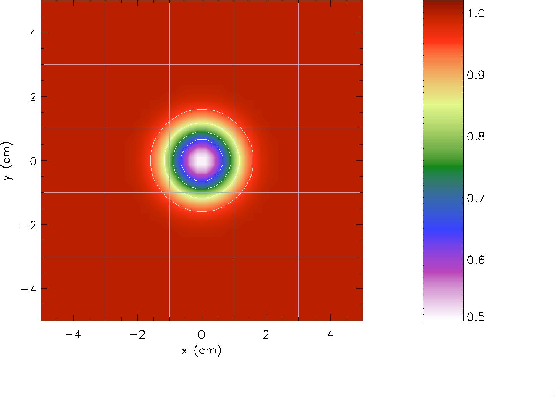
\includegraphics[width=5in]{IsentropicVortex1}}
\end{center}
\caption{\label{Fig:iv1} Density at $t=0.0$ for the isentropic vortex 
problem. Shown are the initial condition and the exact solution
at $t=10.0, 20.0, \ldots$.}
\end{figure}

A numerical simulation using the PPM scheme was run to illustrate
such errors. The simulation used the same grid shown in
\figref{Fig:iv1} with the same contour levels and color values. The
grid is intentionally coarse and the evolution time long to make
numerical errors visible.  The vortex is represented by
approximately 8 grid points in each coordinate direction and is
advected diagonally with respect to the grid.  At solution times of
$t=10, 20, \ldots$, \etc, the vortex should be back at its initial
location.

\figref{Fig:iv2} shows the solution at $t=50.0$; only slight
differences are observed. The density distribution is almost
radially symmetric, although the minimum density has risen to
$0.0537360$. Accumulating dispersion error is clearly visible at
$t=100.0$ (\figref{Fig:iv3}), and the minimum density is now
$0.601786$.
\begin{figure}
\begin{center}
{\leavevmode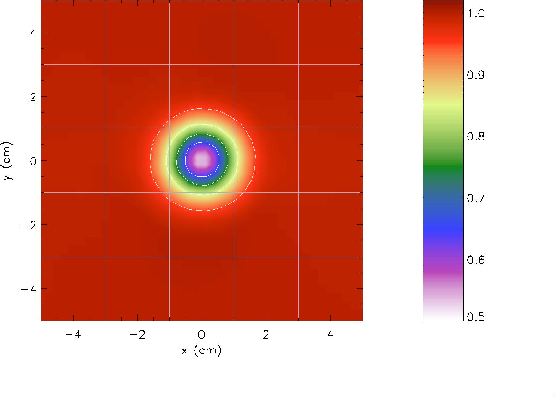
\includegraphics[width=5in]{IsentropicVortex2}}
\end{center}
\caption{\label{Fig:iv2} Density at $t=50.0$ for the isentropic
vortex problem.}
\end{figure}

\begin{figure}
\begin{center}
{\leavevmode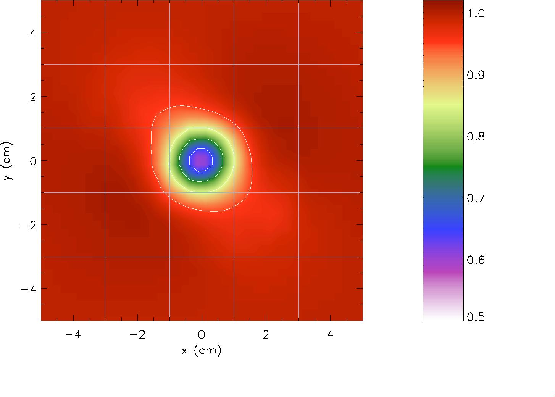
\includegraphics[width=5in]{IsentropicVortex3}}
\end{center}
\caption{\label{Fig:iv3} Density at $t=100.0$ for the isentropic
vortex problem.}
\end{figure}

\figref{Fig:iv4} shows the density near $y=0.0$ at three simulation
times. The black line shows the initial condition. The red line
corresponds to $t=50.0$ and the blue line to $t=100.0$. For the
later two times, the density is not radially symmetric. The lines
plotted are just representative profiles for those times, which give
an idea of the magnitude and character of the errors.
\begin{figure}
\begin{center}
{\leavevmode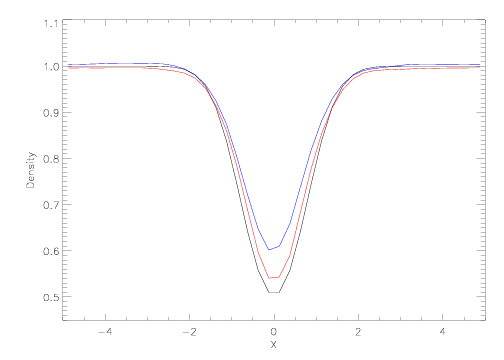
\includegraphics[width=5in]{IsentropicVortex4}}
\end{center}
\caption{\label{Fig:iv4} Representative density profiles for the isentropic
vortex near $y=0.0$ at $t=0.0$ (black), $t=50.0$ (red), and $t=100.0$ (blue).}
\end{figure}

 % This section was added by Lynn Reid from info provided by Alan Calder.
% she has several figures but cannot determine which one is which described below.
% hence this whole section is removed.
%
%% Then someone enable the section again. Then Klaus commented it out again
%% after talking to Anshu, since the figures are still not included. - KW

% \subsubsection{Isentropic Vortex with Particles}
% 
% The problem consists of an isentropic vortex either
% at rest relative to the center of the mesh or propagating across the
% mesh. The tracer particle verification tests with this problem consisted
% of propagating particles with the flow and measuring the error of the
% particle positions relative to the initial conditions. We note that
% measuring the error of the particle positions with the vortex evolving
% also measures the error in the vortex itself as it hydrodynamically
% evolves.
% 
% The isentropic vortex simulation domain as set up for these tests
% is a square, $-5.0 \mathrm{cm} \leq x, y \leq 5.0 \mathrm{cm}$.
% The ambient conditions are $u_{\infty}=1.0 cms $, $v_{\infty} = 1.0 cms $,
% and $T_{\infty} = 1.0 \mathrm{K}$.   The equations of \eqref{Eqn:isentropic_three} hold,
% with initial conditions as given before.
% The flow field is initialized by computing cell averages of the
% conserved variables: each average is approximated by averaging
% over $10^2$ subintervals in the cell. The simulations have periodic boundary
% conditions and time step is fixed.
% 
% The first test of the tracer particles was a consistency test between
% particles propagating in a static vortex and particles propagating in
% a vortex moving diagonally across the grid. \figref{fig:isen01}
% shows the initial velocity distribution for the stationary vortex. The
% moving vortex has an additional constant velocity added that moves the
% vortex diagonally across the grid. Also shown are points indicating the
% initial positions of three test particles. The particles were initially
% 0.2608, 0.7680, and 3.8732 cm from the center of the vortex. The metric
% for comparison in this test was the total velocity of each particle. The
% location of each particle determines its initial velocity, and ideally,
% the particles would maintain exactly the same total velocity over the
% course of the simulation.
% 
% \figref{fig:isen02} shows the velocity of the three test particles
% for both the static and moving vortex cases for 5 s. for a simulation on
% a $128 \times 128$ cell mesh. The velocity of the moving vortex particles
% has the constant translational velocity subtracted.  Also, the particles
% initially have zero velocity and obtain their velocity from the mesh at
% the first time step, and the initial zero velocities have been omitted
% from the plot for clarity. In the figure, the black lines indicate
% the the tracer particle velocities in the static vortex simulation,
% and the gray lines indicate the corrected tracer particle velocities
% in the moving vortex case.  The velocities show good agreement between
% the static and moving vortex simulations and also remain very close
% to constant during the course of the simulation.  In the static vortex
% case, maximum deviation of the radius of any particle reached only 0.3\%
% over the 5 s evolution.
% 
% The next series of tests consisted of resolution studies in space and time. In
% these tests, particles near the center of the vortex were propagated for one
% orbit of the vortex while measuring the radius of the orbit. Ideally, the radius
% of the orbit would remain constant. \figref{fig:isen03} plots the change in
% radius vs.\ time for tracer particles initially 0.261 cm from the center
% of the vortex in simulations on a $128 \times 128$ cell
% simulation mesh at decreasing time steps. The results show that while it
% remains relatively small, the error does not converge with decreasing time
% step.



%===============================================================================
\section{Gravity Test Problems}


\subsection{Homologous Dust Collapse}
\label{Sec:SimulationDustCollapse}

The homologous dust collapse problem \code{DustCollapse}
is used to test the ability
of the code to solve self-gravitating problems in which the flow
geometry is spherical and gas pressure is negligible. The problem was
first described by Colgate and White (1966) and has been used by
M\"onchmeyer and M\"uller (1989) to test hydrodynamical schemes in
curvilinear coordinates.  We solve this problem using a 3D Cartesian
grid.

The initial conditions consist of a uniform sphere of radius $r_0$ and
density $\rho_0$ at rest.  The pressure $p_0$ is taken to be constant and
very small
\begin{equation}
p_0 \ll {4\pi G\over\gamma}\rho_0^2 r_0^2\ .
\end{equation}
We refer to such a nearly pressureless fluid as `dust'. A perfect-gas
equation of state is used, but the value of $\gamma$ is not significant.
Outflow boundary conditions are used for the gas, while isolated boundary
conditions are used for the gravitational field.

The collapse of the dust sphere is self-similar; the cloud should remain
spherical with uniform density as it collapses. The radius of the cloud,
$r(t)$, should satisfy
\begin{equation}
\label{Eqn:dust radius}
\left({8\pi G\over 3}\rho_0\right)^{1/2} t =
\left(1-{r(t)\over r_0}\right)^{1/2}\left({r(t)\over r_0}\right)^{1/2} +
\sin^{-1}\left(1-{r(t)\over r_0}\right)^{1/2}
\end{equation}
(Colgate \& White 1966).
Thus. we expect to test three things with this problem: the ability of the
code to maintain spherical symmetry during an implosion (in particular,
no block boundary effects should be evident); the ability of the code to
keep the density profile constant within the cloud; and the ability of the
code to obtain the correct collapse factor. The second of these is particularly
difficult, because the edge of the cloud is very sharp and because the
Cartesian grid breaks spherical symmetry most dramatically at the center of the
cloud, which is where all of the matter ultimately ends up.

Results of a \code{DustCollapse} run using Flash-X 3.0 appear in
\figref{Fig:dust_flash3}, which shows plots of density and the X
component of velocity in menacing color scheme. The values are plotted
at the end of the run from an X-Y plane in the center of the physical
domain; density is in logarithmic scale. This run used a resolution of
$128^3$, and the results were compared against a similar run using
Flash-X 2.5.  We have also included figures from an earlier higher
resolution run using Flash-X2 which used $4^3$ top-level blocks and
seven levels of refinement, for an effective resolution of $2048^3$.
In both the runs, the multipole Poisson solver was used with a maximum
multipole moment $\ell=0$. The initial conditions used $\rho_0 =
10^9$~g~cm$^{-3}$ and $r_0 = 6.5\times10^8$~cm. In \figref{Fig:dust
collapse}a, the density, pressure, and velocity are scaled by
$2.43\times10^9$~g~cm$^{-3}$, $2.08\times10^{17}$~dyn~cm$^{-2}$, and
$7.30\times10^9$~cm~s$^{-1}$, respectively. In \figref{Fig:dust
collapse}b they are scaled by $1.96\times10^{11}$~g~cm$^{-3}$,
$2.08\times10^{17}$~dyn~cm$^{-2}$, and
$2.90\times10^{10}$~cm~s$^{-1}$. Note that within the cloud, the
profiles are very isotropic, as indicated by the small dispersion in
each profile. Significant anisotropy is only present for low-density
material flowing in through the Cartesian boundaries. In particular,
it is encouraging that the velocity field remains isotropic all the
way into the center of the grid; this shows the usefulness of
refining spherically symmetric problems near $r=0$. However, as
material flows inward past refinement boundaries, small ripples
develop in the density profile due to interpolation errors. These
remain spherically symmetric but increase in amplitude as they are
compressed. Nevertheless, they are still only a few percent in
relative magnitude by the second frame.  The other numerical effect
of note is a slight spreading at the edge of the cloud.  This does
not appear to worsen significantly with time. If one takes the
radius at which the density drops to one-half its central value as
the radius of the cloud, then the observed collapse factor agrees
with our expectation from \eqref{Eqn:dust radius}. Overall our
results, including the numerical effects, agree well with those of
M\"onchmeyer and M\"uller (1989).

This problem is configured to use the perfect-gas
equation of state (\code{gamma}) with \code{gamma} set to 1.67 and
is run in a three-dimensional box.  The problem uses the specialized
refinement marking routine supplied under the Grid interface of
\code{Grid_markRefineSpecialized} which refines blocks
containing the center of the cloud.

\begin{figure}[t]
\begin{center}
\subfigure[]{\label{Fig:dust_dens}
  \includegraphics[width=3.0in]{DustCollapse_dens}
}
\subfigure[]{\label{Fig:dust_velx}
  \includegraphics[width=3.0in]{DustCollapse_velx}
}
\caption{\label{Fig:dust_flash3}
  XY plane of Density (a) and X component of Velocity (b) are shown at the center of the domain
for the \code{DustCollapse} problem. The velocity is in normal scale, while density is logscale.
}
\end{center}
\end{figure}

\begin{figure}[t]
\begin{center}
\subfigure[]{\label{Fig:dust1}
  \includegraphics[width=3.0in]{DustCollapse1}
}
\subfigure[]{\label{Fig:dust2}
  \includegraphics[width=3.0in]{DustCollapse2}
}
\caption{\label{Fig:dust collapse}
  Density (black), pressure (red), and velocity (blue) profiles
  in the homologous dust collapse problem at (a) $t=0.0368$~sec
  and (b) $t=0.0637$~sec. The density, pressure, and velocity are
  scaled as discussed in the text.
}
\end{center}
\end{figure}
\clearpage

%\vfill
%\eject

%-------------------------------------------------------------------------------

\subsection{MacLaurin}
\label{Sec:SimulationMacLaurin}
The gravitational potential at the surface of, and inside a homogeneous spheroid
called a ``MacLaurin spheroid'' is expressible in terms of analytical functions.
This handy result was first determined by MacLaurin (1801), and later summarized by,
amongst others, Chandrasekhar (1989).  These properties allow validation of 
the \flashx gravitational solvers against the analytical solutions.

As a test case, an oblate ($a_1 = a_2 > a_3$) Maclaurin spheroid, of a constant density $\rho = 1$ 
in the interior, and $\rho = \epsilon \rightarrow 0$ outside (in \flashx 
\rpi{Grid/smlrho} is used). 
The spheroid is motionless and in hydrostatic equilibrium. 
The gravitational potential of such object is analytically 
calculable, and is:
\begin{equation}
\phi({\bf x}) = \pi G \rho \left[ 2A_1 a_1^2 - A_1(x^2+y^2) + A_3(a_3^2-z^2) \right] \ ,
\end{equation}
for a point inside the spheroid. Here 
\begin{eqnarray}
A_1 &=& \frac{\sqrt{1-e^2}}{e^3} \sin^{-1}e - \frac{1-e^2}{e^2}\ , \\
A_3 &=& \frac{2}{e^2} - \frac{2\sqrt{1-e^2}}{e^3} \sin^{-1}e\ ,
\end{eqnarray}
where $e$ is the ellipticity of a spheroid:
\begin{equation}
e = \sqrt{1 - \left( \frac{a_3}{a_1} \right) ^2}\ .
\end{equation}
For a point outside the spheroid, potential is: 
\begin{equation}
\phi({\bf x}) = \frac{2a_3}{e^2} \pi G \rho \left[a_1 e \tan^{-1}h - \frac{1}{2} \left( (x^2+y^2) 
                \left( \tan^{-1}h - \frac{h}{1+h^2} \right) + 2z^2 (h-\tan^{-1}h) \right) \right]\ ,
\end{equation}
where 
\begin{equation}
h = \frac{a_1 e}{\sqrt{a_3^2 + \lambda}}\ ,
\end{equation}
and $\lambda$ is the positive root of the equation 
\begin{equation}
\frac{x^2}{a_1^2 + \lambda} + \frac{y^2}{a_2^2 + \lambda} + \frac{z^2}{a_3^2 + \lambda} = 1\ .
\end{equation}

This test is also useful because the spheroid has spherical symmetry in the X--Y plane, 
but also lack of such symmetry in X--Z and Y--Z planes.
The density distribution of the spheroid is shown in \figref{Fig:Maclaurin_density}.
Spherical symmetry is simple to reproduce with a solution using multipole expansion.
However, the non-symmetric solution requires
an infinite number of multipole moments, while the code 
calculates solution up to a certain $l_{max}$, specified by the user
as runtime parameter \rpi{Grid/mpole_lmax}. The error is thus expected to be dominated 
by the first non-zero term in the remainder of expansion. Also, the solution for any point inside 
the spheroid is the sum of monopole and dipole moments. 

\begin{figure}[!ht]
\begin{center}
{\leavevmode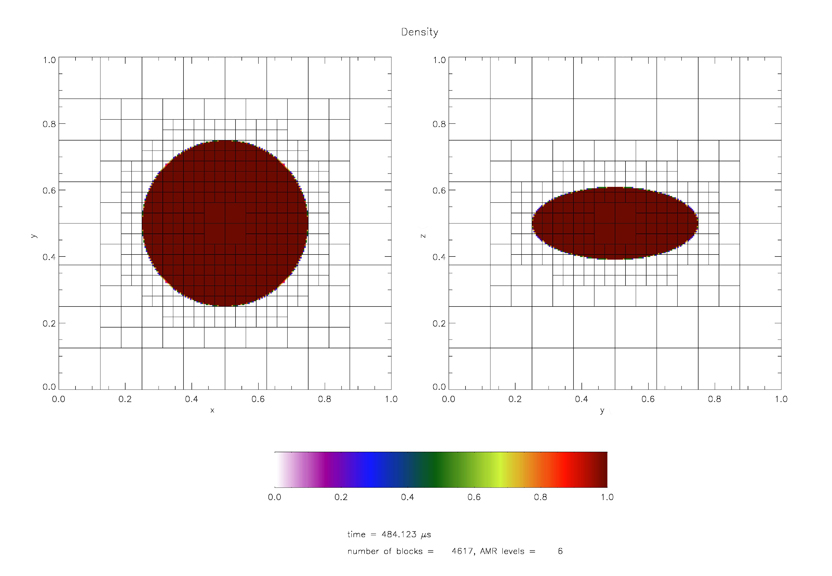
\includegraphics[width=150mm]{Maclaurin_density}}
\end{center}
\label{Fig:Maclaurin_density}
\caption{Density of the MacLaurin spheroid (left X--Y plane, right Y--Z plane) with ellipticity
$e=0.9$.  The \flashx block structure is shown on top.}
\end{figure}

The simulation is calculated on a MacLaurin spheroid with eccentricity $e=0.9$; several other values for eccentricity were tried with results qualitatively the same.
All tests used 3D Cartesian coordinates. 
The gravitational potential is calculated on an adaptive mesh, and the relative error is investigated: 
\begin{equation}
\label{Eqn:Maclaurin_error}
\epsilon = \left| \frac{\phi_{\rm analytical} - \phi_{\rm Flash-X}}{\phi_{\rm analytical}} \right|
\end{equation}
from zone to zone. 

\begin{table*}[!ht]
	\centering
		\begin{tabular}{|r|r|r|r|r|r|}
			\hline
      $l_{max}$&min$(\epsilon)$&max$(\epsilon)$&relative $L^2_{in}$ norm& relative $L^2_{out}$ norm&approx. time $[s]$\\
      \hline
      0&$4.5\ 10^{-6}$&$0.182$&$7.1\ 10^{-2}$&$6.8\ 10^{-2}$&$9.8$\\
      1&$4.5\ 10^{-6}$&$0.182$&$7.1\ 10^{-2}$&$6.8\ 10^{-2}$&$14.5$\\
      2&$9.8\ 10^{-6}$&$0.062$&$1.4\ 10^{-2}$&$1.7\ 10^{-2}$&$34.7$\\
      4&$1.0\ 10^{-8}$&$0.026$&$4.0\ 10^{-3}$&$5.0\ 10^{-3}$&$55.4$\\
      6&$6.1\ 10^{-9}$&$0.013$&$1.6\ 10^{-3}$&$2.5\ 10^{-3}$&$134.9$\\
      8&$7.8\ 10^{-9}$&$0.007$&$8.7\ 10^{-4}$&$1.2\ 10^{-3}$&$210.2$\\
      10&$6.7\ 10^{-9}$&$0.004$&$5.5\ 10^{-4}$&$7.0\ 10^{-4}$&$609.7$\\
      \hline
		\end{tabular}
	\caption{Minimal and maximal relative error in all zones of the simulation, calculated 
	         using \eqref{Eqn:Maclaurin_error}. Last row is approximate time for one full timestep (gravity only).}
	\label{tab:multipoles}
\end{table*}

As expected, increasing spatial resolution improves the solution quality, but here we focus on 
how the solution depends on the choice of $l_max$, the cutoff 
$\ell$ in \eqref{Eqn:Multipole_poisint2}. In \figref{Fig:Maclaurin_mpole0}--\ref{Fig:Maclaurin_mpole0}
the gravitational potential for the Maclaurin 
spheroid, the \flashx solution, and relative errors for several $l_{max}$'s are shown. 
A similar figure produced for $l_{max}=1$ shows no difference from \figref{Fig:Maclaurin_mpole0},
indicating that the last dipole term in the multipole expansion does not contribute to the accuracy
of the solution but does increase computational cost.
Because gravity sources are all of the same sign, and the symmetry of the 
problem, all odd-$l$ moments are zero: reasonable, physically motivated values for 
setting \rpi{Grid/mpole_lmax} should be an even number. 

In the X--Y plane, where the solution is radially symmetric, the first monopole term is enough to qualitatively capture the correct
potential. As expected, the error is the biggest on the spheroid boundary, 
and decreases both outwards and inwards. Increasing the maximum included moment reduces errors.
However, in other non-symmetric planes, 
truncating the potential to certain $l_{max}$ leads to an error whose leading term will be 
the spherical harmonic of order $l_{max}+2$, as can be nicely seen in the lower right sections of 
\figref{Fig:Maclaurin_mpole0} -- \ref{Fig:Maclaurin_mpole10}.
Increasing $l_{max}$ reduces the error, but also increases the required time for computation.
This computational increase is not 
linear because of the double sum in \eqref{Eqn:multipole potential}. 
Luckily, convergence is rather fast, and already 
for $l_{max} = 4$, there are only few zones with relative error bigger than 1\%, while for the most of the computational domain the error is several orders of magnitude less. 

\begin{figure}
\begin{center}
{\leavevmode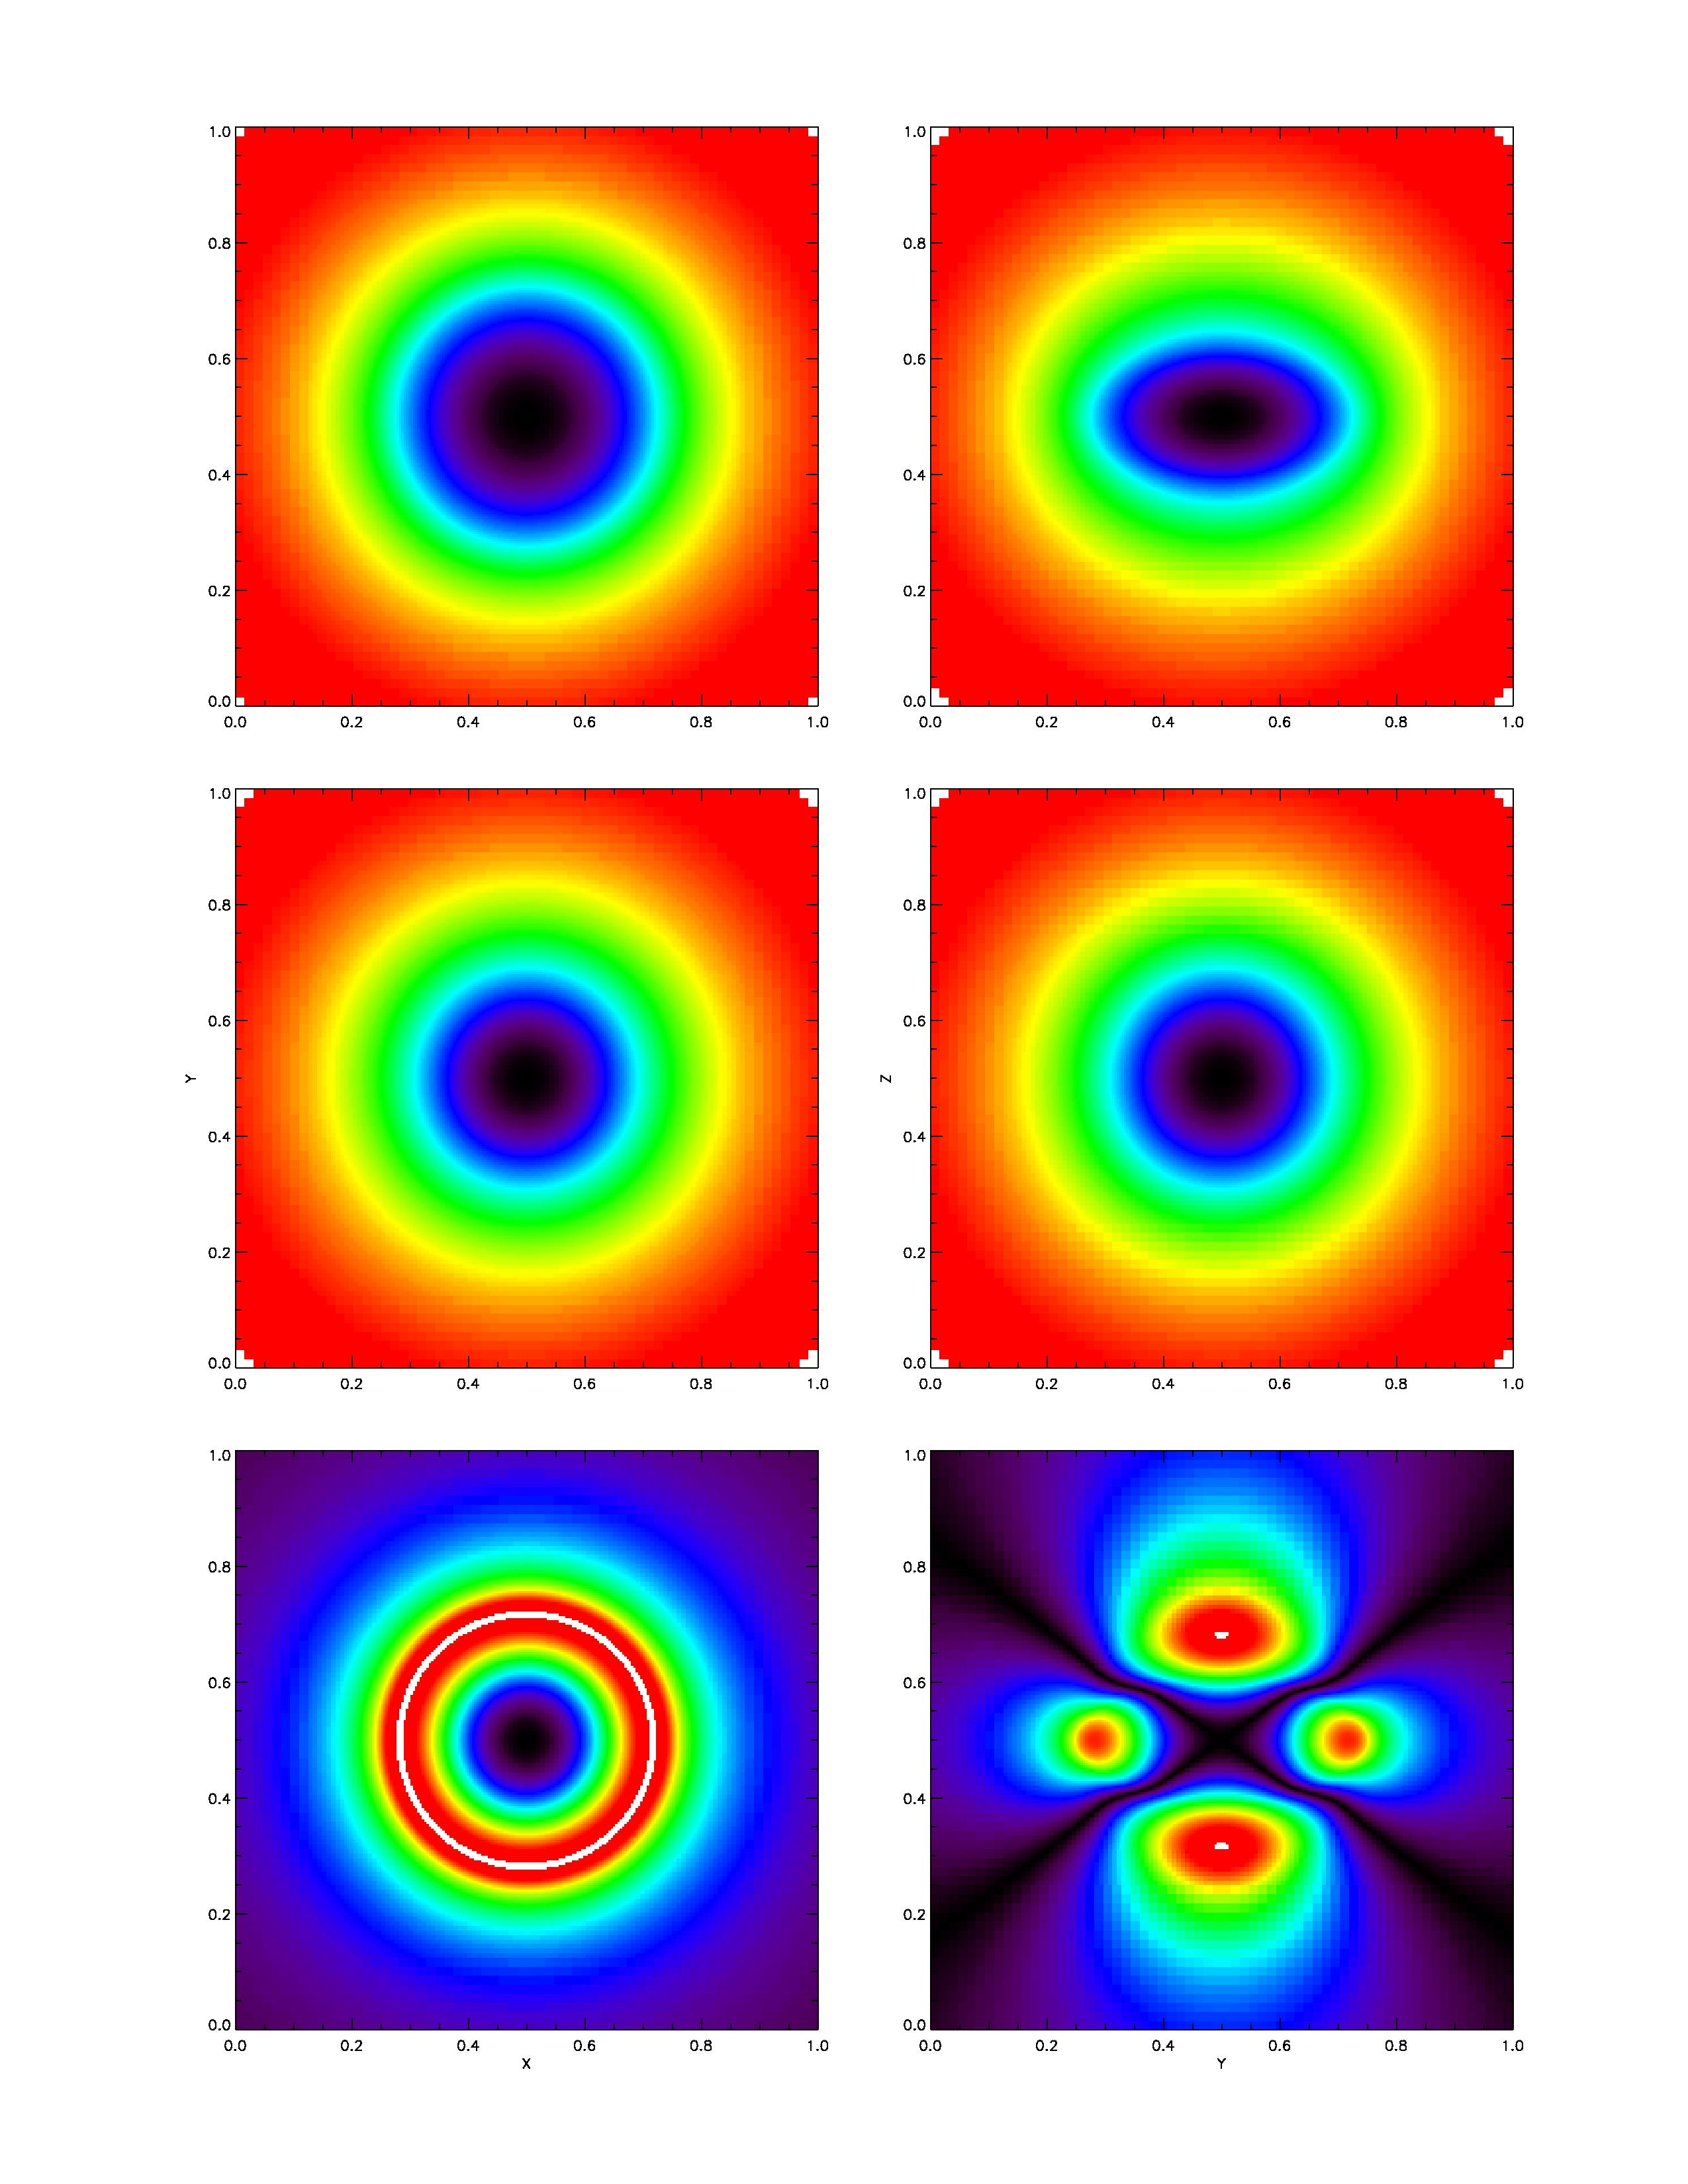
\includegraphics[width=140mm]{Maclaurin_mpole0}}
\end{center}
\caption{Maclaurin spheroid: $l_{max} = 0$, 6 refinement levels. Left column is X--Y plane, 
                cut through z=0.5, right column is Y--Z plane cut through x=0.5 .
                From top to bottom: analytical solution for the gravitational potential introduced on 
                Flash-X grid; solution of Flash-X multipole solver; relative error.}
\label{Fig:Maclaurin_mpole0}
\end{figure}


\begin{figure}
\begin{center}
{\leavevmode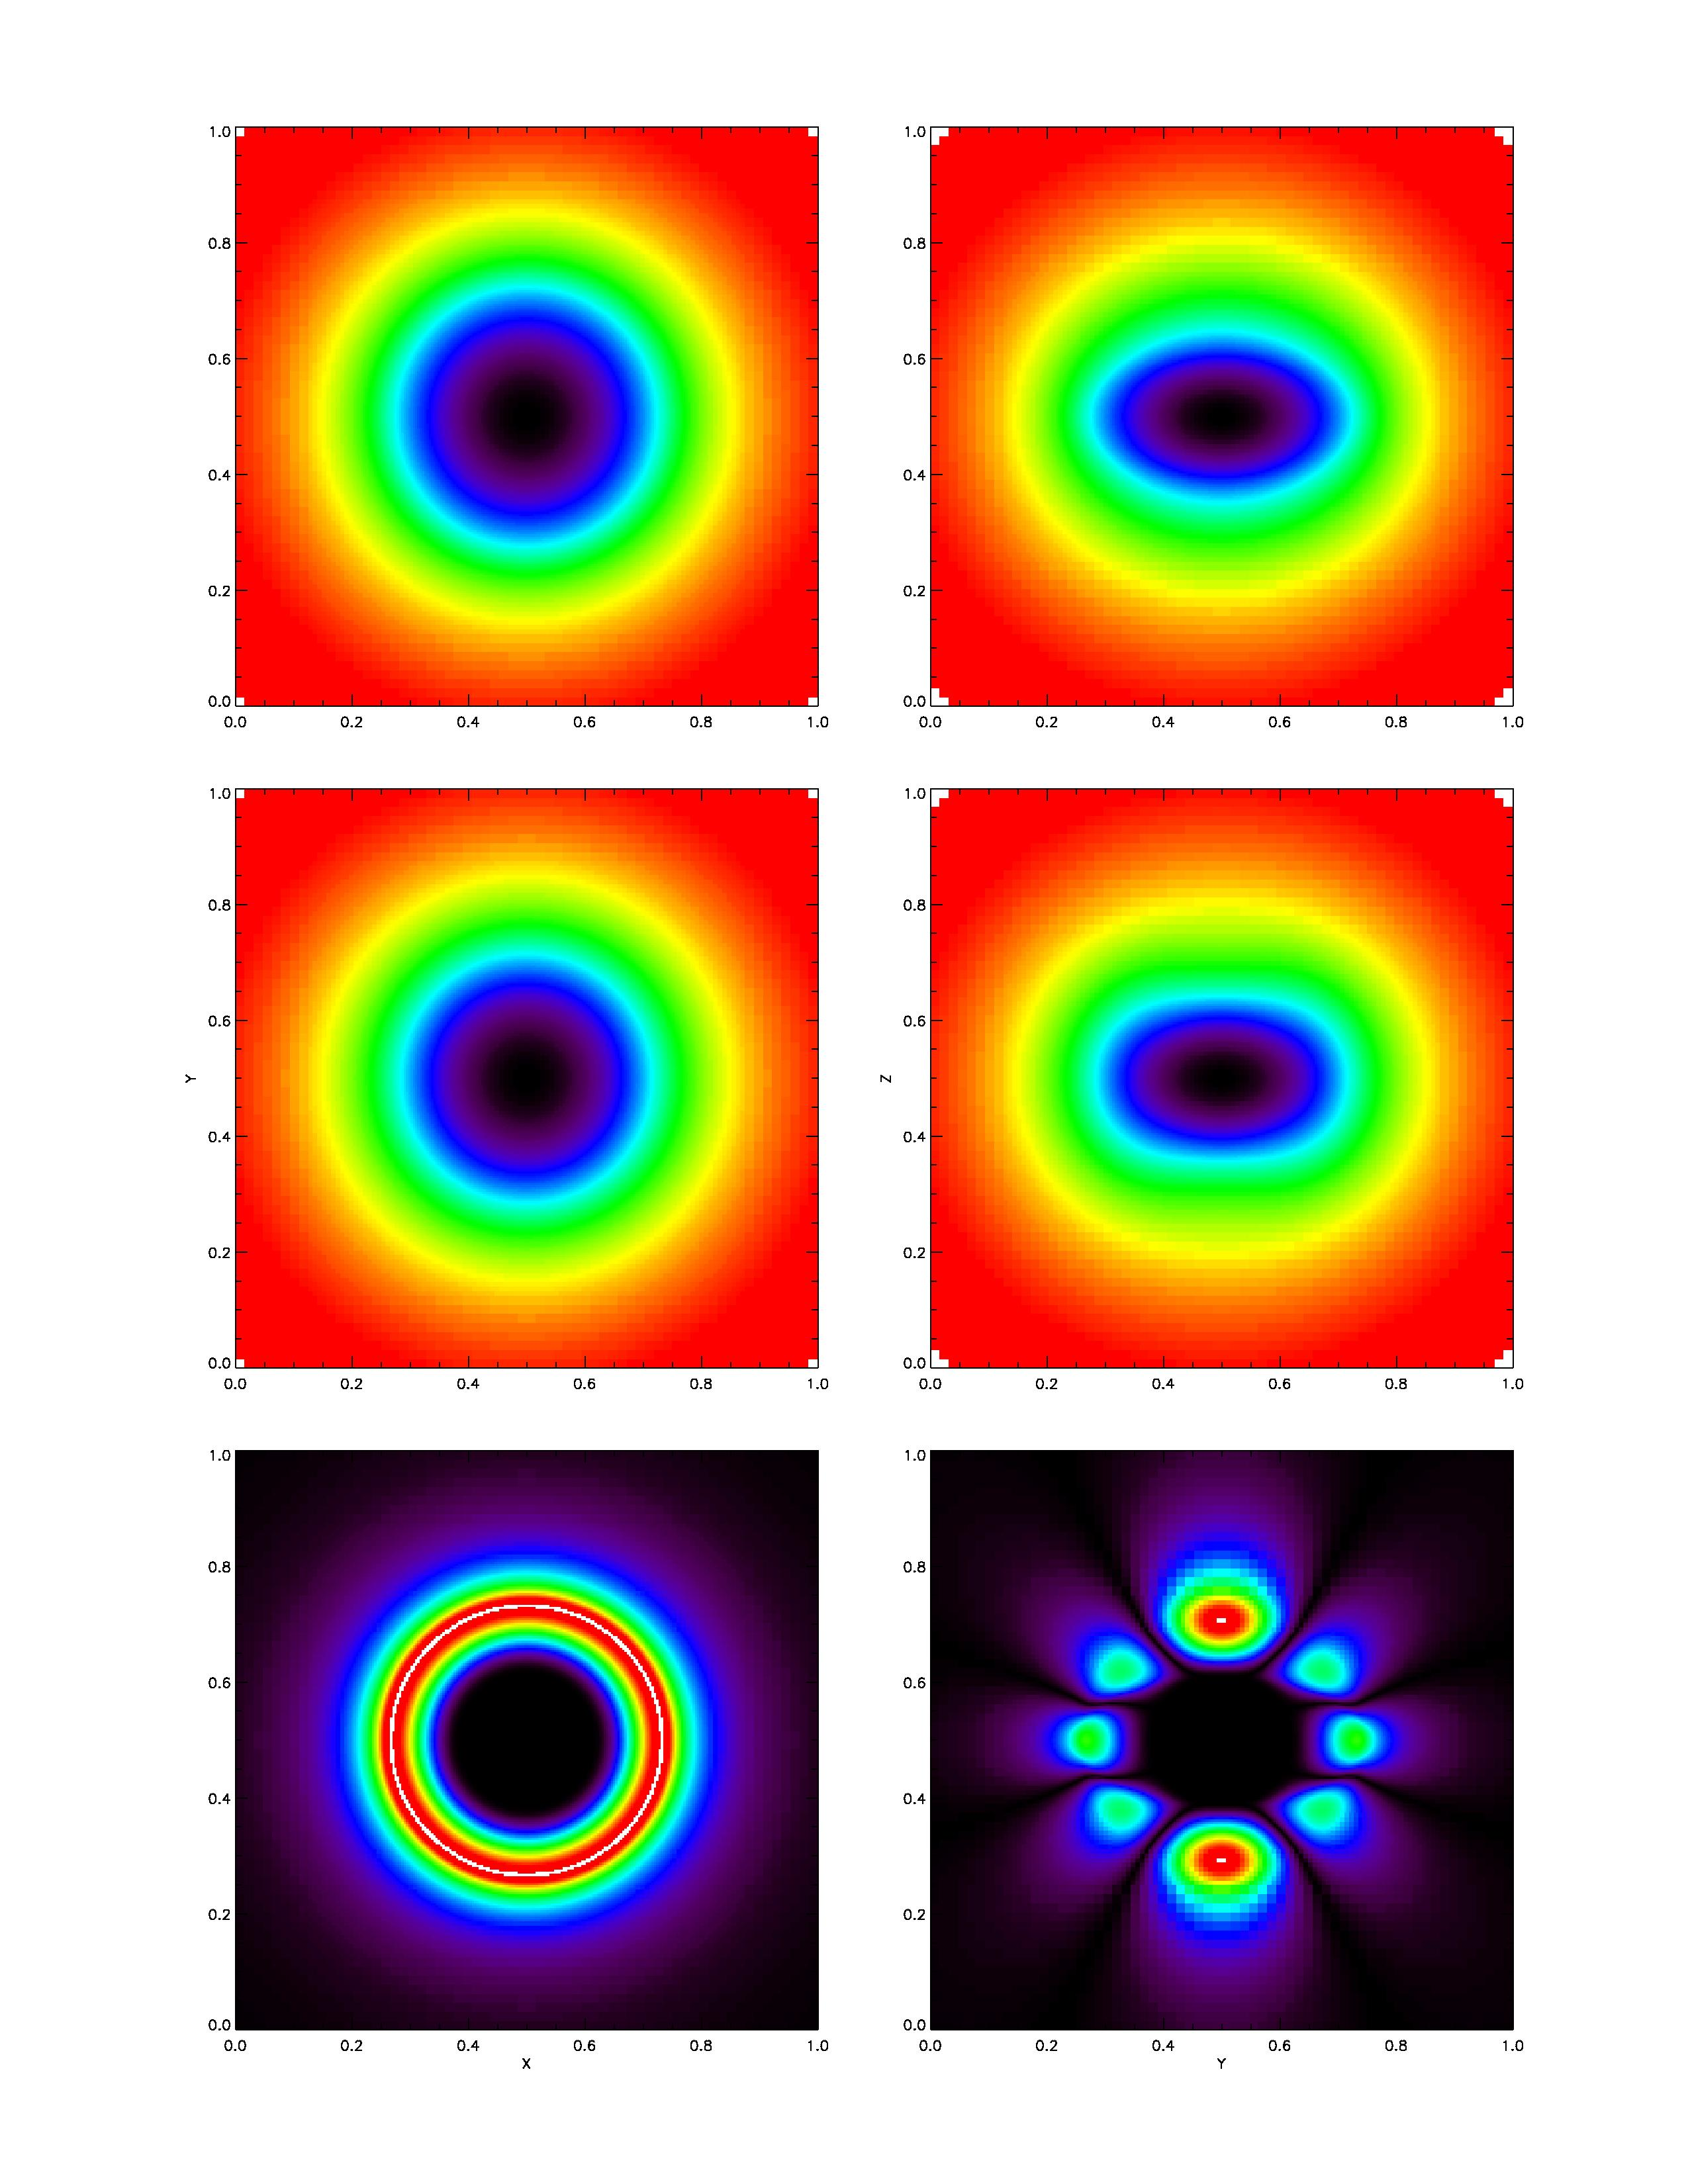
\includegraphics[width=140mm]{Maclaurin_mpole2}}
\end{center}
\caption{Maclaurin spheroid: $l_{max} = 2$, 6 refinement levels. Left column is X--Y plane, 
                cut through z=0.5, right column is Y--Z plane cut through x=0.5 . 
                From top to bottom: analytical solution for the gravitational potential introduced on 
                Flash-X grid; solution of Flash-X multipole solver; relative error.}
\label{Fig:Maclaurin_mpole2}
\end{figure}


\begin{figure}
\begin{center}
{\leavevmode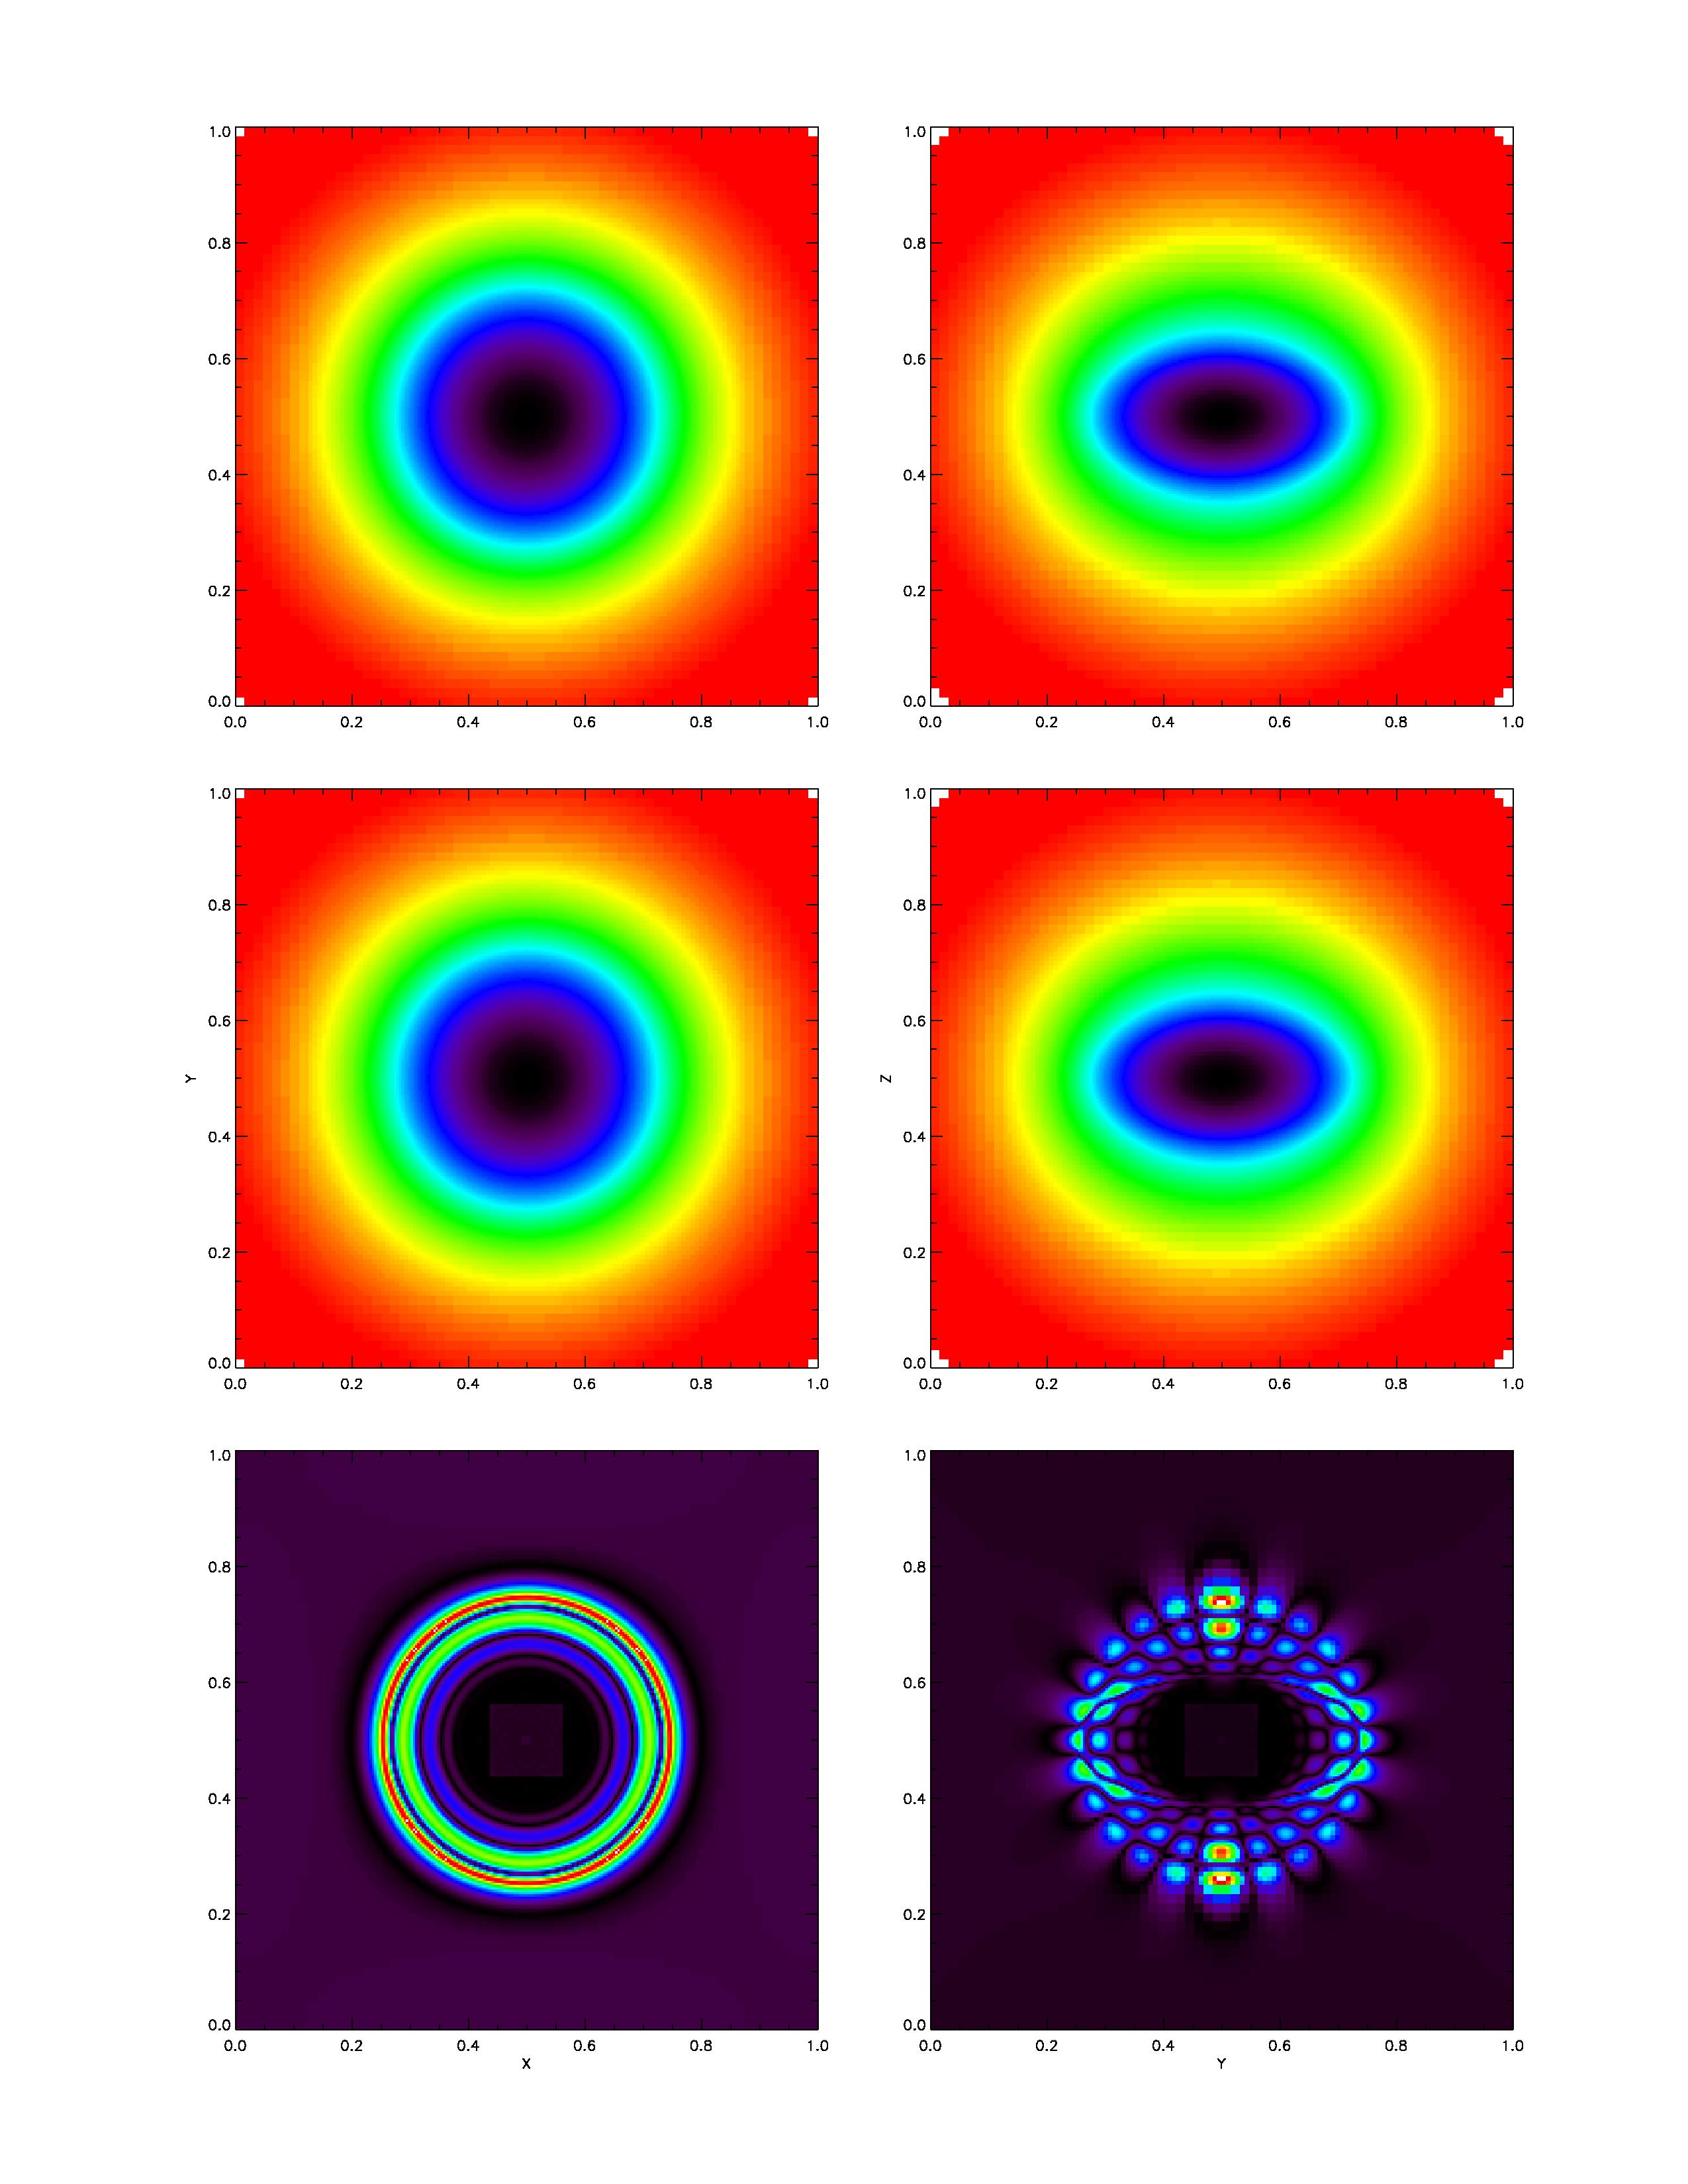
\includegraphics[width=140mm]{Maclaurin_mpole10}}
\end{center}
\caption{Maclaurin spheroid: $l_{max} = 10$, 6 refinement levels. Left column is X--Y plane, 
                cut through z=0.5, right column is Y--Z plane cut through x=0.5 .
                From top to bottom: analytical solution for the gravitational potential introduced on 
                Flash-X grid; solution of Flash-X multipole solver; relative error.}
\label{Fig:Maclaurin_mpole10}
\end{figure}



\section{Burn Test Problem}

\subsection{Cellular Nuclear Burning}
\label{Sec:SimulationCellular}

The \code{Cellular} Nuclear Burning problem is used primarily to test the function of
the Burn simulation unit.  The problem exhibits regular steady-state behavior
and is based on one-dimensional models described by Chappman (1899) and
Jouguet (1905) and Zel'dovich (Ostriker 1992), von Neumann (1942), and
Doring (1943).  This problem is solved in two dimensions.  A complete description
of the problem can be found in a recent paper by Timmes, Zingale et al\. (2000).



A 13 isotope $\alpha$-chain plus heavy-ion reaction network is used
in the calculations.  A definition of what we mean by an
$\alpha$-chain reaction network is prudent. A strict $\alpha$-chain
reaction network is only composed of ($\alpha$,$\gamma$) and
($\gamma$,$\alpha$) links among the 13 isotopes $^4$He, $^{12}$C,
$^{16}$O, $^{20}$Ne, $^{24}$Mg, $^{28}$Si, $^{32}$S, $^{36}$Ar,
$^{40}$Ca, $^{44}$Ti, $^{48}$Cr, $^{52}$Fe, and $^{56}$Ni.  It is
essential, however, to include ($\alpha$,p)(p,$\gamma$) and
($\gamma$,p)(p,$\alpha$) links in order to obtain reasonably accurate
energy generation rates and abundance levels when the temperature
exceeds $\sim$ 2.5$\times$10$^{9}$ K. At these elevated temperatures
the flows through the ($\alpha$,p)(p,$\gamma$) sequences are faster
than the flows through the ($\alpha$,$\gamma$) channels.  An
($\alpha$,p)(p,$\gamma$) sequence is, effectively, an
($\alpha$,$\gamma$) reaction through an intermediate isotope.  In our
$\alpha$-chain reaction network, we include 8 ($\alpha$,p)(p,$\gamma$)
sequences plus the corresponding inverse sequences through the
intermediate isotopes $^{27}$Al, $^{31}$P, $^{35}$Cl, $^{39}$K,
$^{43}$Sc, $^{47}$V, $^{51}$Mn, and $^{55}$Co by assuming steady state
proton flows.  \begin{comment}This strategy permits inclusion of
($\alpha$,p)(p,$\gamma$) sequences without explicitly evolving the
proton or intermediate isotope abundances. Thus, the $\alpha$-chain
reaction network in Flash-X includes not just ($\alpha$,$\gamma$) and
($\gamma$,$\alpha$) links, but also links through the
($\alpha$,p)(p,$\gamma$) and ($\gamma$,p)(p,$\alpha$) sequences.  How
well this small reaction network mimics the nuclear energy generation
rate given by a large 489 isotope reaction network is analyzed in
(Timmes, Hoffman, \& Woosley 2000).\end{comment}

The two-dimensional calculations are performed in a planar geometry of size 256.0 cm by 25.0 cm.
The
initial conditions consist of a constant density of 10$^7$ g
cm$^{-3}$, temperature of 2$\times$10$^{8}$ K, composition of pure
carbon X($^{12}$C)=1, and material velocity of $v_{x}=v_{y}$= 0 cm
s$^{-1}$.  Near the x=0 boundary the initial conditions are perturbed to the
values given by the appropriate Chapman-Jouguet solution: a density of
4.236$\times$10$^7$ g cm$^{-3}$, temperature of 4.423$\times$10$^9$ K,
and material velocity of $v_{x}$ = 2.876$\times$10$^8$ cm s$^{-1}$.
Choosing different values
or different extents of the perturbation simply change how long it
takes for the initial conditions to achieve a near ZND state, as well as
the block structure of the mesh.  Each block contains 8 grid points in the
x-direction, and 8 grid points in the y-direction. The default parameters for
cellular burning are given in \tblref{Tab:cellularParameters}.


\begin{center}
\begin{longtable}{lllp{3in}}
\caption{ Runtime parameters used with the
\code{Cellular} test problem.} \\
\label{Tab:cellularParameters}
Variable    & Type      & Default   & Description\\
\hline
\code{xhe4} & real          & 0.0           & Initial mass fraction of He4\\
\code{xc12} & real          & 1.0           & Initial mass fraction of C12\\
\code{xo16} & real          & 0.0           & Initial mass fraction of O16\\
\code{rhoAmbient}  & real   & 1$\times$10$^{7}$     & Density of cold
                                  upstream material.\\
\code{tempAmbient} & real   & 2$\times$10$^{8}$     & Temperature of cold
                                  upstream material.\\
\code{velxAmbient} & real   & 0.0                   & X-velocity of cold
                                  upstream material.\\
\code{rhoPerturb}  & real & 4.236$\times$10$^{7}$ & Density of the post shock
                                                   material.\\
\code{tempPerturb} & real & 4.423$\times$10$^{9}$ & Temperature of the post
                            shock material.\\
\code{velxPerturb} & real & 2.876$\times$10$^{8}$ & X-velocity of the post shock
                                                   material.\\
\code{radiusPerturb} & real & 25.6 & Distance below which the perturbation is
                      applied.\\
\code{xCenterPerturb} & real & 0.0 & X-position of the origin of the
                     perturbation\\
\code{yCenterPerturb} & real & 0.0 & Y-position of the origin of the
                     perturbation\\
\code{zCenterPerturb} & real & 0.0 & Z-position of the origin of the
                     perturbation\\
\code{usePseudo1d} & logical & \code{.false.} & Defaults to a spherical
                        configuration.  Set to
                        \code{.true.} if you want to
                        use a 1d configuration, that
                        is copied in the y and z
                        directions.\\
\code{noiseAmplitude} & real & 1.0$\times$10$^{-2}$ & Amplitude of the white
                                                      noise added to the
                              perturbation.\\
\code{noiseDistance} & real & 5.0 & The distance above the starting radius to
                                    which white noise is added.\\

\hline
\end{longtable}
\end{center}


% \begin{figure}
% \begin{center}
% {\leavevmode\includegraphics[width=4in]{Cellular_initial_conditions}}
% \end{center}
% \caption{\label{Fig:initial} Initial conditions of the cellular nuclear burning problem}
% \end{figure}

The initial conditions and perturbation given above ignite the nuclear
fuel, accelerate the material, and produce an over-driven detonation
that propagates along the x-axis.  The initially over-driven
detonation is damped to a near ZND state on short time-scale.  After
some time, which depends on the spatial resolution and boundary
conditions, longitudinal instabilities in the density cause the planar
detonation to evolve into a complex, time-dependent structure. \figref{Fig:end_run} shows the pressure field of the detonation after
\hbox{1.26$\times$10$^{-7}$ s}.  The interacting transverse wave
structures are particularly vivid, and extend about 25 cm behind the
shock front.  \figref{Fig:det_front} shows a close up of this traverse
wave region.  Periodic boundary conditions are used at the walls parallel to
the y-axis while reflecting boundary conditions were used for the walls
parallel to the x-axis.

\begin{figure}
\begin{center}
{\leavevmode\includegraphics[width=4in]{Cellular_end_run}}
\end{center}
\caption{\label{Fig:end_run} Steady-state conditions of the \code{Cellular}
nuclear burn problem.}
\end{figure}


\begin{figure}
\begin{center}
{\leavevmode\includegraphics[width=4in]{Cellular_det_front}}
\end{center}
\caption{\label{Fig:det_front} Close-up of the detonation front in steady-state for
the \code{Cellular} nuclear burn problem.}
\end{figure}

\subsection{The HydroStatic Test Problem}
\label{Sec:HydroStatic}
The \code{Hydrostatic} problem tests the basic function of
hydrostatic boundary conditions implemented in the
\unit{Grid} unit, in connection with a \unit{Hydro} implementation.
It is essentially a 1D problem, but can
be configured as 1 1D, 2D, or 3D setup.
It can be easily modified to include additional physical effects,
by including additional code units in the setup.

In its default configuration, \code{HydroStatic} is set up with constant \unit{Gravity}.
The domain is initialized with density, pressure, \etc, fields representing
an analytical solution of the hydrostatic problem with the given
gravitational acceleration, essentially following the
barometric formula.

This initial condition is then evolved in time.  Ideally, the solution would remain
completely static, and nothing should move.  The deviation from this ideal
behavior that occurs in practice is a measure of the quality of the discretization of
the initial condition, of the hydrodynamics implementation, and of the boundary
conditions.  The effect of the latter, in particular, can be examined by
visualizing artifacts that develop near the boundaries (in particular, velocity
artifacts), and studying their dependence on the choice of boundary condition variant.

